\chapter{Particle in a Central Potential. The Hydrogen Atom}\footnote{Cohen}
In thsi chapter, we shall consider the quantum mechanical properties of a particle placed in a central potential [that is, a potential $V(r)$ which depends only on the distance $r$ from the origin]. This problem is closely related to the study of angular momentum. As we shall know, the fact that $V(r)$ es invariant under any rotation about the origin means that the Hamiltonian $H$ of the particle conmutes with the three components of the orbital angular momentum operator $\vb{L}$. This cosiderably simplifies the determination of the eigenfunctions and eigenvalues of $\vb{L}^2$ and $L_z$ as well.



\section{Statioanary states of a particle in a central potential}
In this section, we consider a (spinless) particle of mass $\mu$, subjected to a central force derived from the potential $V(r)$ (the center of force is chosen as the origin).
\subsection{Outline of the problem}
\subsubsection{Review of some classical results}
The force acring on the classical particle situated at the point $M$ (with $\vb{OM}=\vb{r}$) is equal to:
\begin{equation}\label{A-1}
	\vb{F}=-\nabla V(r)=-\dv{V}{r}\frac{\vb{r}}{r}
\end{equation}
$\vb{F}$ is always directed towards $O$,  and its mimentum with respect to this point is therefore always zero. If:
\begin{equation}\label{A-2}
	\vb{\mathcal{L}}=\vb{r}\times\vb{p}
\end{equation}
is the angular momentum of the particle with respecto to $O$, the anfular momentum theorem implies that:
\begin{equation}\label{A-3}
	\dv{\vb{\mathcal{L}}}{t}=\vb{0}
\end{equation}
$\vb{\mathcal{L}}$ is therefore a \textit{constant of the motion}, so that the particle's trajectory is necessarily situated in the plane passing through $O$ and perpendicular to $\vb{\mathcal{L}}$.

\begin{figure}[h]
	\begin{center}
		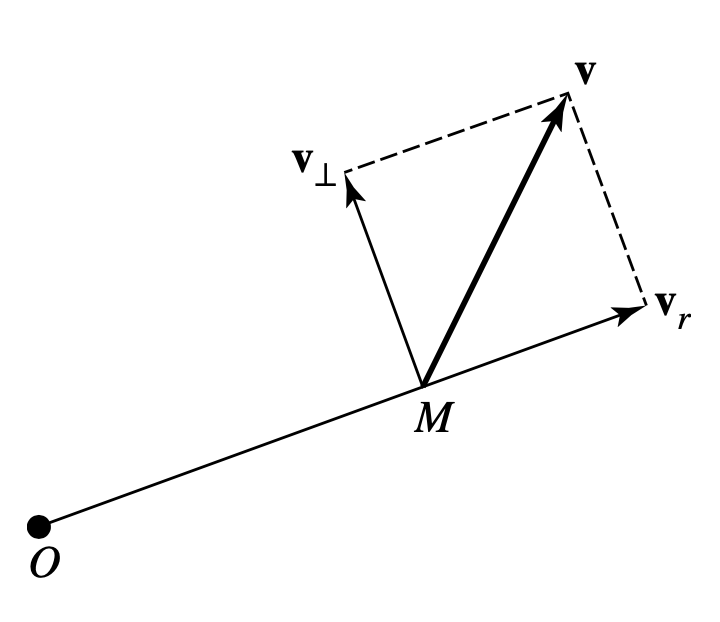
\includegraphics[scale=0.6]{fig/fig1-A-cohen.png}
		\caption{Radial component $\vb{v}_r$ and tangential component $\vb{v}_\perp$ of a particle's velocity.}
		\label{fig:1-a-cohen}
	\end{center}	
\end{figure}

Now let us consider Fig. \ref{fig:1-a-cohen} the position (denoted by $\vb{OM}=\vb{r}$) and velocity $\vb{v}$ of the particle at the instant $t$. Thw two vectors $\vb{r}$ and $\vb{v}$ lie in the plane of the trajectory and the velocity $\vb{v}$ can be decomposed into the radial component $\vb{v}_r$ (along the axis defined by $\vb{r}$) and the tangential component $\vb{v}_\perp$ (along the axis perpendicular to $\vb{r}$). The radual velocity, the algebraic value of $\vb{v}_r$, is the time derivative of the distance of the particle from the point $O$:
\begin{equation}\label{A-4}
	v_r=\dv{r}{t}
\end{equation}
The tangential velociry can be expressed in term of $r$ and the angular momentum $\vb{\mathcal{L}}$, since:
\begin{equation}\label{A-5}
	|\vb{r}\times\vb{v}|=r|\vb{v}_\perp|
\end{equation}
so that the modulus of the angular momentum $\vb{\mathcal{L}}$ is equal to:
\begin{equation}\label{A-6}
	|\vb{\mathcal{L}}|=|\vb{r}\times\mu\vb{v}|=\mu r|\vb{v}_\perp|
\end{equation}
The total energy of the particle:
\begin{equation}\label{A-7}
	E=\frac{1}{2}\mu\vb{v}^2+V(r)=\frac{1}{2}\mu \vb{v}_r^2+\frac{1}{2}\mu \vb{v}_\perp^2+V(r)
\end{equation}
can be written:
\begin{equation}\label{A-8}
	E=\frac{1}{2}\mu\vb{v}_r^2+\frac{\vb{\mathcal{L}}^2}{2\mu r^2}+V(r)
\end{equation}
The classical Hamiltonian if the system is then:
\begin{equation}\label{A-9}
	\mathcal{H}=\frac{p_r^2}{2\mu}+\frac{\vb{\mathcal{L}}^2}{2\mu r^2} + V(r)
\end{equation}
where:
\begin{equation}\label{A-10}
	p_r=\mu\dv{r}{t}
\end{equation}
is the conjugate momentum of $r$,  and $\vb{\mathcal{L}}^2$ must be expressed in terms of the variables $r, \theta, \varphi$ and their conjugate momenta $p_r,p_\theta,p_\varphi$. One finds:
\begin{equation}\label{A-11}
	\vb{\mathcal{L}}^2=p_\theta ^2 +\frac{1}{\sin^2\theta}p_\varphi^2
\end{equation}
In expression (\ref{A-9}), the kinetic energy is broken into two terms: the radial kinetic energy and the kinetic energy of rotation about $O$ . The reason is that, since $V(r)$ is independent of $\theta$ and $\varphi$ in this case, the angular variables and their conjugate momenta appear only in the $\vb{\mathcal{L}}^2$ term. In fact, if we are interested in the evolution of $r$, we can use the fact that $\vb{\mathcal{L}}$ is a constant of the motion, and replace $\vb{\mathcal{L}}^2$ by a constant in expression (\ref{A-9}). The Hamiltonian $\mathcal{H}$  then appears as a function only of the radial variables $r$ and $p_r$ ( $\vb{\mathcal{L}}^2$ plays the role of a parameter), and the result is a differential equation involving only one variable, $r$:
\begin{equation}\label{A-12a}
	\dv{p_r}{t}=\mu\dv[2]{r}{t}=-\pdv{\mathcal{H}}{r}
\end{equation}
that is:
\begin{equation}\label{A-12b}
	\mu\pdv[2]{r}{t}=\frac{\vb{\mathcal{L}}^2}{\mu r^2}-\dv{V}{r}
\end{equation}
It is just as if we had a one-dimensional problem (with $r$ varyng only between $0$ and $+\infty$), with a particle of mass $\mu$ subjected to the "efective potential":
\begin{equation}\label{A-13}
	V_{eff}(r)=V(r)+\frac{\vb{\mathcal{L}}^2}{2\mu r^2}
\end{equation}
We shall see that the situation is analogous in quantum mechanics.


\subsubsection{The quantum mechanical Hamiltonian}
In quantum mechanics, we want to solve the eigenvalue equation of the Hamiltonian $\mathcal{H}$, the observable associated with the total energy. This equation is written, in the $\{\ket{\vb{r}}\}$ representation:
\begin{equation}\label{A-14}
	\left[-\frac{\hbar^2}{2\mu}\Delta +V(r)\right]\varphi(\vb{r}) = E\varphi(\vb{r})
\end{equation}
Since the potential $V$ depends only on the distance  $r $of the particle from the origin, spherical coordinates are best adapted to the problem. We therefore express the Laplacian $\Delta$ in spherical coordinates \footnote{Expression (\ref{A-15}) gives the Laplacian only for non-zero $r$. This is because of the privileged position of the origin in spherical coordinates; it can be seen, moreover, that expression (\ref{A-15}) is not defined for $r=0$.}
\begin{equation}\label{A-15}
	\Delta = \frac{1}{r}\pdv[2]{r}r+\frac{1}{r^2}\left(\pdv[2]{\theta} +\frac{1}{\tan\theta}\pdv{\theta}+\frac{1}{\sin^2\theta}\pdv[2]{\varphi}\right)
\end{equation}
andd look for eigenfucntions $\varphi(\vb{r})$ that are functions of the variables $r,\theta,\varphi$.















